% mnras_template.tex 
%
% LaTeX template for creating an MNRAS paper
%
% v3.0 released 14 May 2015
% (version numbers match those of mnras.cls)
%
% Copyright (C) Royal Astronomical Society 2015
% Authors:
% Keith T. Smith (Royal Astronomical Society)

% Change log
%
% v3.0 May 2015
%    Renamed to match the new package name
%    Version number matches mnras.cls
%    A few minor tweaks to wording
% v1.0 September 2013
%    Beta testing only - never publicly released
%    First version: a simple (ish) template for creating an MNRAS paper

%%%%%%%%%%%%%%%%%%%%%%%%%%%%%%%%%%%%%%%%%%%%%%%%%%
% Basic setup. Most papers should leave these options alone.
\documentclass[fleqn,usenatbib]{mnras}

% MNRAS is set in Times font. If you don't have this installed (most LaTeX
% installations will be fine) or prefer the old Computer Modern fonts, comment
% out the following line
\usepackage{newtxtext,newtxmath}
% Depending on your LaTeX fonts installation, you might get better results with one of these:
%\usepackage{mathptmx}
%\usepackage{txfonts}

% Use vector fonts, so it zooms properly in on-screen viewing software
% Don't change these lines unless you know what you are doing
\usepackage[T1]{fontenc}
\usepackage{subfig} %for figure subplot
\usepackage{graphicx}
\usepackage[flushleft]{threeparttable}
\usepackage{xspace}



%%%%%%%%%%%%%%%%%%%%%%%%%%%%%%%%%%%%%%%%%%%%%%%%%%%%%%%%%%%%%%%%%%%
% my commands
\newcommand{\lcdm}{$\Lambda$CDM}
\newcommand{\hst}{{\it HST}}
\newcommand{\efr}{$R_{\mathrm{eff}}$}
\newcommand{\galfit}{{\sc Galfit}}
\newcommand{\mbh}{$\mathcal M_{\rm BH}$}
\newcommand{\lhost}{$L_{\rm host}$}
\newcommand{\mr}{$Mag_{\rm ~R}$}
\newcommand{\halpha}{H$_{\alpha}$}
\newcommand{\Hb}{H$_{\beta}$}
\newcommand{\sersic}{S\'ersic}
\newcommand{\lenstronomy}{{\sc Lenstronomy}}
\newcommand{\reff}{{$R_{\mathrm{eff}}$}}
\newcommand{\kmsMpc}{km~s$^{\rm -1}$~Mpc$^{\rm -1}$}
\newcommand{\kms}{\ifmmode{\,\rm{km}\, \rm{s}^{-1}}\else{$\,$km$\,$s$^{-1}$}\fi}
\newcommand{\sigstar}{{$\sigma_*$}}
\newcommand{\mstar}{{$M_*$}}
\newcommand{\Mgii}{Mg$_{\rm II}$}
\newcommand{\Civ}{C$_{\rm IV}$}
%\newcommand{\farcs}{\mbox{\ensuremath{.\!\!^{\prime\prime}}}}% fractional arcsecond symbol: 0.''0
\newcommand{\sam}{\texttt{SAM}}
\newcommand{\mbii}{\texttt{MBII}}
%%%%%%%%%%%%%%%%%%%%%%%%%%%%%%%%%%%%%%%%%%%%%%%%%%%%%%%%%%%%%%%%%%%
\newcommand{\ding}[1]{\textcolor{red}{[{\bf Xuheng}: #1]}}
\newcommand{\todo}[1]{\textcolor{red}{[{\bf Todo}: #1]}}  
\newcommand{\red}[1]{{ \textcolor{red}{#1}}}
\newcommand{\blue}[1]{{ \textcolor{blue}{#1}}}
\newcommand{\pink}[1]{{ \textcolor{magenta}{#1}}}

% Allow "Thomas van Noord" and "Simon de Laguarde" and alike to be sorted by "N" and "L" etc. in the bibliography.
% Write the name in the bibliography as "\VAN{Noord}{Van}{van} Noord, Thomas"
\DeclareRobustCommand{\VAN}[3]{#2}
\let\VANthebibliography\thebibliography
\def\thebibliography{\DeclareRobustCommand{\VAN}[3]{##3}\VANthebibliography}


%%%%% AUTHORS - PLACE YOUR OWN PACKAGES HERE %%%%%

% Only include extra packages if you really need them. Common packages are:
\usepackage{graphicx}	% Including figure files
\usepackage{amsmath}	% Advanced maths commands
\usepackage{amssymb}	% Extra maths symbols

%%%%%%%%%%%%%%%%%%%%%%%%%%%%%%%%%%%%%%%%%%%%%%%%%%

%%%%% AUTHORS - PLACE YOUR OWN COMMANDS HERE %%%%%

% Please keep new commands to a minimum, and use \newcommand not \def to avoid
% overwriting existing commands. Example:
%\newcommand{\pcm}{\,cm$^{-2}$}	% per cm-squared

%%%%%%%%%%%%%%%%%%%%%%%%%%%%%%%%%%%%%%%%%%%%%%%%%%

%%%%%%%%%%%%%%%%%%% TITLE PAGE %%%%%%%%%%%%%%%%%%%

% Title of the paper, and the short title which is used in the headers.
% Keep the title short and informative.
\title[Mass relations by lensed AGN hosts]{The Mass Relations between Supermassive Black Holes and Their Host Galaxies using Eight Strongly Lensed AGN Systems.}

% The list of authors, and the short list which is used in the headers.
% If you need two or more lines of authors, add an extra line using \newauthor
\author[X. Ding et al.]{
Xuheng Ding,$^{1}$\thanks{E-mail: dxh@astro.ucla.edu}
Tommaso Treu,$^{1}$
Simon Birrer,$^{1, 2}$
Dominique Sluse,\newauthor
Chris Fassnacht,
Matthew W. Auger,
Kenneth C. Wong,
Sherry H. Suyu,\newauthor
Takahiro Morshita,
and et al. $^{3}$
\\
% List of institutions
$^{1}$Department of Physics and Astronomy, University of California, Los Angeles, CA, 90095-1547, USA\\
$^{2}$Kavli Institute for Particle Astrophysics and Cosmology and Department of Physics, Stanford University, Stanford, CA 94305, USA\\
$^{3}$xxx
}

% These dates will be filled out by the publisher
\date{Accepted XXX. Received YYY; in original form ZZZ}

% Enter the current year, for the copyright statements etc.
\pubyear{2020}

% Don't change these lines
\begin{document}
\label{firstpage}
\pagerange{\pageref{firstpage}--\pageref{lastpage}}
\maketitle

% Abstract of the paper
\begin{abstract}
Strong lensed AGN has been considered as a unique tool to exam the correlations between the mass of the supermassive Black Hole and its host galaxies. In this work, we have adopted eight strongly lensed system from the H0LiCOW collaboration. The deep \hst\ data and adopt the \lenstronomy\ to reconstruct the image of the source. Using the reconstructed brightness of the host galaxy, we infer the host galaxy stellar mass based on the assumed stellar population. 
The \mbh\ are estimated using the board emission line. We compare our inference to the ones in the literature and find a consistent result. The consistent scaling resolutions derived from our sample confirm the evolution conclusion and confirm the the power of using strong lensed AGNs. The sample of the data are supposed to increase rapidly.
\end{abstract}

% Select between one and six entries from the list of approved keywords.
% Don't make up new ones.
\begin{keywords}
galaxies: evolution -- galaxies: active -- gravitational lensing: strong
\end{keywords}

%%%%%%%%%%%%%%%%%%%%%%%%%%%%%%%%%%%%%%%%%%%%%%%%%%

%%%%%%%%%%%%%%%%% BODY OF PAPER %%%%%%%%%%%%%%%%%%

\section{Introduction}
The tight correlations between the masses (\mbh) of supermassive black holes (BHs) and their host galaxies properties including stellar mass (\mstar), stellar velocity dispersion ($\sigma_*$) and luminosity (\lhost), known as scaling relations, are usually considered as a result of their co-evolution.

The origin of these relations is till unclear so far. In theory, cosmological simulations of structure formation are able to reproduce the local tight relation based on physical mechanism by invoking active galactic nucleus (AGN) feedback as the physical connection or having them share a common gas supply. On the other hand, without any physical coupling, the pure statistical convergence by galaxy mergers alone could also reproduce the observed correlations at local universe. It is crucial to extend the correlation studies to higher redshift and understand their evolution as a function of redshift. Recently, \citet{Ding2020} measured the scaling relations at redshift range of $1.2<z<1.7$ based on a sample of 32 AGNs using \hst/WFC3. Comparing to the published samples at local and intermediate redshift range, they confirm the an evolution scenario that the growth of BHs evolution predates than the host galaxy bulge. In the following up work, \citet{Ding2020b} used the measurements of the high-$z$ AGNs and compare to numerical simulations including the hydrodynamic simulation MassiveBlackII (MBII) and a semi-analytic model (SAM). The tightness of the scaling relation at high-$z$ supports the hypothesis that AGN feedback as a promising driver for the scaling correlations. A larger sample at higher redshift would be even more beneficial to confirm this scenario.

Benefiting from the gravitational lensing magnification and stretching effect, strong lensed AGNs provide a unique tool to make progress in this study (ref[Peng2006]), 
provided that the lens modelling is accurate. \citet{Ding2017a} has carried out extensive and realistic simulations tests based on the deep \hst\ observations for a sample of eight lens systems in H0LiCOW collaboration. This work has confirm the reconstruction of the lensed host galaxy properties can be recovered with better precision and accuracy than the typical \mbh\ uncertainty. As a following up effort, \citet{Ding2017b} has applied the advanced techniques to two strongly lensed systems to study their \mbh-\lhost\ relations and obtained consistent results to the ones in the literature.

In this work, we aim to make progress by completing the analysis of the entire eight systems. We have developed an independent approach to achieve a one-step inference of the host photometry. We adopt the a set of extended modelling choices to assure the accuracy of our measurements. Moreover, we comparing our new measurements to the ones which have been modelled by the H0LiCOW collaboration to make the cross check. 3/8 of our objects have multi-band \hst\ imaging and we are able to infer their host color to assess an accurate inference of the stellar mass. The extended range of the eight systems would help us to make a direct comparison to the latest measurements by \citet{Ding2020}. We also adopt a class of self-consistent recipes to recalibrate the \mbh\ of our sample.

This paper is organized as follows xxx. Zeropoint are defined in the AB systems. A Chabrier initial mass function (IMF) is employed consistently. 

\section{Sample Selection}\label{sec:sample_select}
We adopt the eight lens systems from our H0LiCOW collaboration including HE0435$-$1223, RXJ1131$-$1231, WFI2033$-$4723, HE1104$-$1805, SDSS1206$+$4332, SDSS0246$-$0825, HE0047$-$1756 and HS2209$+$1914. For conciseness, we abbreviate each lens name to four digits (e.g., RXJ~1131$-$1231 to RXJ1131). In \citet{Ding2017a}, the simulation exercise has been performed to understand the fidelity of the source reconstruction based on these eight systems and verified that the host inference is trustworthy when its magnitude are brighter than 20 magnitude, 2$-$4 magnitudes dimmer than the AGN. The detailed information of the observational conditions of our eight systems are given in Table~\ref{data_set}. Besides the adopted filter shown therein, some systems also observed by \hst\ by different bands. As will shown in Section~\ref{sec:mstar}, the multi-band information enables us to apply the stellar population, hence a more accurate \mstar\ estimation. 

While we note that our sample size included eight systems, which is a limited sample to constrain the evolution of the scaling relation. In this particular work, we simply aim to plot the scaling relation of our sample and make comparison to the ones in the literature. %[]The comparison sample (32 QSO paper)
We adopt the recent efforts by~\citet{Ding2020}, including 32 AGNs at redshift range $1.2<z<1.9$, 79 intermediate redshift QSO and 55 local measurements. It is worth noticing that they are so far the largest \hst\ imaging AGN samples with redshift range from 1.9 to the local. 
 
\begin{table}
\centering
%\begin{threeparttable}
\caption{Summary of lensed AGN information.}\label{data_set}
\resizebox{9cm}{!}{
     \begin{tabular}{cccccc}
        \hline
Object ID & $z$ & camera & Filter & exposure & pixel scale \\
 & & & & time (s) & (drizzled) \\ \hline
HE0435$-$1223 & 1.69 & WFC3-IR & F160W & 9340 & $0\farcs{}08$ \\
RXJ1131$-$1231 & 0.65 & ACS & F814W & 1980 & $0\farcs{}05$ \\
WFI2033$-$4723 & 1.66 & WFC3-IR & F160W & 26257 & $0\farcs{}08$ \\
SDSS1206$+$4332 & 1.79 & WFC3-IR & F160W & 8457 & $0\farcs{}08$ \\
HE1104$-$1805 & 2.32 & WFC3-IR & F160W & 14698 & $0\farcs{}08$ \\
SDSS0246$-$0825 & 1.68 & WFC3-UVIS & F814W & 8481 & $0\farcs{}03$ \\
HS2209$+$1914 & 1.07 & WFC3-UVIS & F814W & 14238 & $0\farcs{}03$ \\
HE0047$-$1756 & 1.66 & WFC3-UVIS & F814W & 9712 & $0\farcs{}03$ \\
        \hline
     \end{tabular}
    }
\begin{tablenotes}
      \small
      \item Note: $-$ The observational information is presented in~\citet{Ding2017a}.
\end{tablenotes}  
%\end{threeparttable}
\end{table}

To assure the validity of the comparison, we adopt a class of self-consistent recipes as introduced in~\citet{Ding2020} to estimate the \mbh\ of our sample. For the overall systems, we adopt the following virial formalism:
\begin{eqnarray}
\label{recipe}
\log \left(\frac{\mathcal M_{\rm BH}}{M_{\odot}}\right)&~=~& a+b \log \left(\frac{ \rm L _{\lambda_{line}}}{10^{44}{\rm erg~s^{-1}}}\right) \nonumber\\
&~+~& 2 \log \left(\frac{\rm FWHM(line)}{1000 ~{\rm km~s^{-1}}}\right) , 
\end {eqnarray}
%
with a\{\Civ, \Mgii, \Hb\}=\{6.322, 6.623, 6.910\},
b\{\Civ, \Mgii, \Hb\}=\{0.53, 0.47, 0.50\},
$\lambda_{line}$\{\Civ, \Mgii, \Hb\}=\{1350, 3000, 5100\}.
%
Having achieved a consistent cross-calibration, we adopt the board line information from the literature \citep{Sluse2012, Peng2006, Shen2011} to estimate the \mbh. The information are presented in Table~\ref{mbh}. The uncertainty of the \mbh\ are expected as $0.4$~dex.


\begin{table}
\centering
%\begin{threeparttable}
\caption{Summary of lensed \mbh\ estimates.}\label{mbh}
\resizebox{8.5cm}{!}{
     \begin{tabular}{ccccc}
        \hline
Object ID & Line(s) used & FWHM & log($L_\lambda$) & $\log$\mbh \\
& & (\kms) & (${\rm erg~s^{-1}}$) & (M$_{\odot}$) \\ \hline
HE0435 & \Mgii & 4930 & 45.14 & 8.54 \\
RXJ1131 & \Mgii/\Hb & 5630/4545 & 44.29/44.02 & 8.26/8.23 \\
WFI2033 & \Mgii & 3960 & 45.19 & 8.38 \\
SDSS1206 & \Mgii & 5632 & 45.61 & 8.88 \\
HE1104 & \Civ & 6004 & 46.18 & 9.03 \\
SDSS0246 & \Mgii & 3700 & 45.19 & 8.32 \\
HS2209 & xxx & xxx & xxx &  xxx  \\
HE0047 & \Mgii & 4145 & 45.59 & 8.60 \\
        \hline
     \end{tabular}
    }
\begin{tablenotes}
      \small
      \item Note: $-$ The reference for the board line information. For SDSS1206, we follow Birrer2018~ref[] and consider the magnification effect to correct the L.
\end{tablenotes}  
%\end{threeparttable}
\end{table}

\section{surface photometry with lensing technique}
We present the lensed host galaxy source reconstruction to derive their intrinsic photometry in this section. Our lensed AGN systems are from the H0LiCOW project, and the lens models of four systems have been derived with host galaxies reconstructed ref[]. Aiming at time-delay cosmography, these works focused on deriving the precise and accurate lens models, while the reconstruction of the host galaxy is only a by-product. In this paper, we apply the state-of-the-art lens modeling technique and dedicate to recovering the photometry of the host galaxy. As will show, approach would allow us to obtain a one-step host magnitude defined by \sersic\ profile, which is consistent to the definitions in the literature. %Furthermore, for cross check purpose, we compare our inference to the reconstructions by the previous works.

\subsection{Model Choice}
We carry out the fitting process to subtract the central AGN light, constrain the lens model, and reconstruct the host galaxy in the source plan, simultaneously.
For all the systems, we assume the photometry of the galaxies (including the lensing galaxy and source galaxy) is described by the 2-D elliptical \sersic\ profile. We start with a single \sersic\ and consider to use two \sersic\ if any significant residual indicate a multiply component. For single \sersic\ case, we set the prior of the \sersic\ index value $n$ between $[0.5-5.0]$ to avoid unphysical inference\footnote{It has been studied in ref[] that this prior value would result in a consistent host magnitude inference as to fix n to its true value.}. The bright AGNs are unsolved and modelled by a scaled point spread function (PSF). We also joint the fitting of the AGN position to the center of its host.
 We adopt the elliptical Power-law model to describe the surface mass density of the deflector; an external shear component is also added.

We employ the imaging modelling tool \lenstronomy~ref[] to perform the fitting task. We following the standard procedure as described by~\citet{Ding2020} to prepare the fitting ingredients including the lensing imaging data, noise level map and the PSF information. The imaging data are drizzled to a higher resolution by setting a Gaussian kernel; the adopted final resolution are listed in Table~\ref{data_set}. We then adopt the {\sc photutils} by Python to model the 2-D global background light using SExtractor algorithm. We then remove the background light and cut the clear image data into postage stamp at a suitable size. We draw the image mask for each systems to define the region in which the pixels would to be included in the likelihood; see Figure~\ref{fig:image_inference}.

For each lens system, we adopt different choices to perform the fitting. The distribution of the fitting inference are assumed to sufficiently cover the truth. We then apply a statistical measurement to weighting for the final inference and estimate the uncertainty level. The different choice of the fitting including the following.
\begin{enumerate}
\item Following common practice, we select all the bright, isolated stars across the image frame of targets to define the PSF. Each selected star is consider as the initial PSF to input to the fitting, which is considered as different choice.
\item The central pixel of the AGNs are very bright and have systematic errors during the interpolation of the subsampled PSF. To avoid overfitting the noise, we adopt two different modelling options: 1)~manually boost the noise estimate in the central area to effectively infinite; 2)~perform the iterative PSF estimation as introduced by ref[].
\item To calculate the ray tracing under a higher resolution grid, the different relative level to the pixel sizes is selected, including [$2\times2$, $3\times3$] pixel$^{-1}$.
\item Using the lensing imaging alone is difficult to constrain the power-law slope. To avoid any overfitting, we fix the slope values during the lens modelling with three optional value $[1.9, 2.0, 2.1]$.
\end{enumerate}

All in all, for one lens system with a number of $N$ initial PSFs, we select in total of $N\times12$ (i.e., $2 \times2 \times3$) different choices of fitting. After  all sets of fittings are completed, we rank their performance of each choice based on their best-fitted $\chi^2$ value. Finally, we adopt the weighting algorithm as introduced by Equations (3)$-$(6) in~\citet{Ding2020}. Since there is no obvious evidence of better perform between QSO mask or PSF iteration, we selected each top-4 fitting by these to choice and combining them equally to derive the final results and to evaluate the uncertainties.

\subsection{Photometry Inference}\label{sec:photometry}
In this subsection, we describe the details of the fitting for each systems and present our inference of the host galaxy photometry.

\subsubsection{HE0435}
The modeling is set up based on the descriptions in the last section. We select 5 isolated stars in this field initial PSFs to input to the fitting with in total of 60 fittings for this system. Based on the top-eight choices, we perform the weighting algorithm and measure the host-to-total flux ratio, host magnitude, effective radius and \sersic\ index. The inference results are shown in Table~\ref{tab:host_measure}, (2)$-$(5) columns.

The lens model inference based on the best-fit result for HE0435 is drawn in Figure~\ref{fig:image_inference}-(a). Not surprisingly, we note that the residual level reveals are appears to be larger than the ones as presented by Ken[] or Simon[]. This is due to the fact that the definition of the host galaxy in our models is a 2-D \sersic\ model which is relatively simple compare to the pixellated reconstruction technique by {\sc Glee} or the shapelet functions as adopted by \lenstronomy. The smooth feature of our model couldn't capture the clumps in the host of the star-forming regions, however, our model is more effective to derive the global host light as function of the \sersic\ which is consistent to measurements in the comparison sample. 

As a cross check, we compare our host magnitude to the measurement in Ding+2017[], in which they model the reconstructed host galaxy as \sersic\ based on Galfit []. The host magnitude measured in that paper is: $mag = 21.75 \pm 0.13$, %, $R_{eff} = 0.82 \pm 0.14$ and $n = 3.94 \pm 0.14$. 
which is slightly fainter than our inference, i.e. $mag = 21.50 \pm 0.35$. The offset is within $1-\sigma$ level.

\begin{figure*}
\centering
\begin{tabular}{c c}
\subfloat[HE0435]{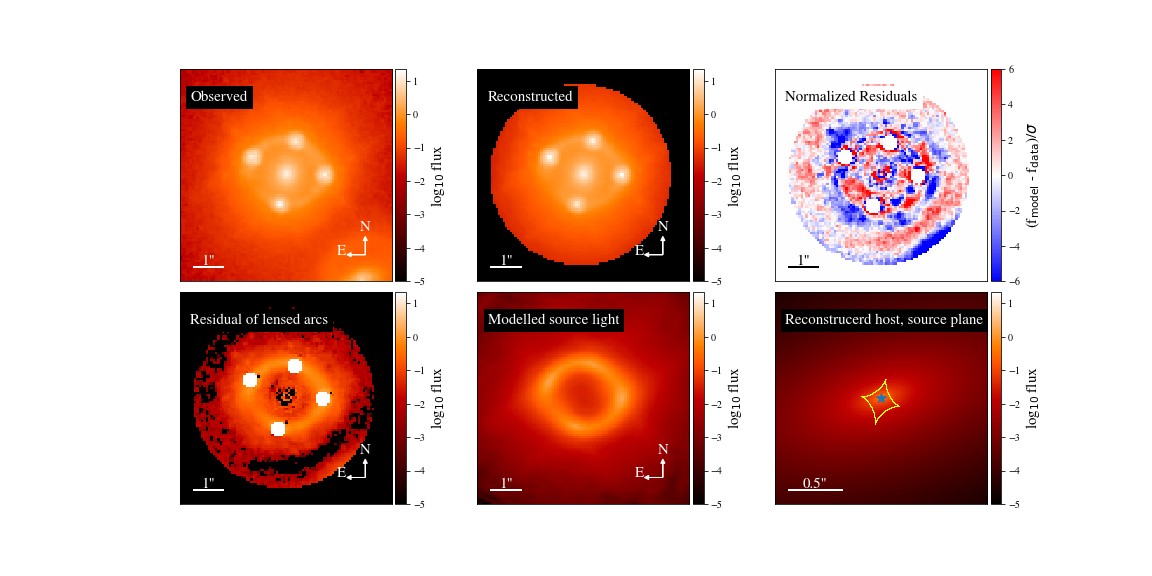
\includegraphics[trim = 40mm 25mm 40mm 25mm, clip, width=0.5\textwidth]{fig/HE0435_inference.png}}&
\subfloat[RXJ1131]{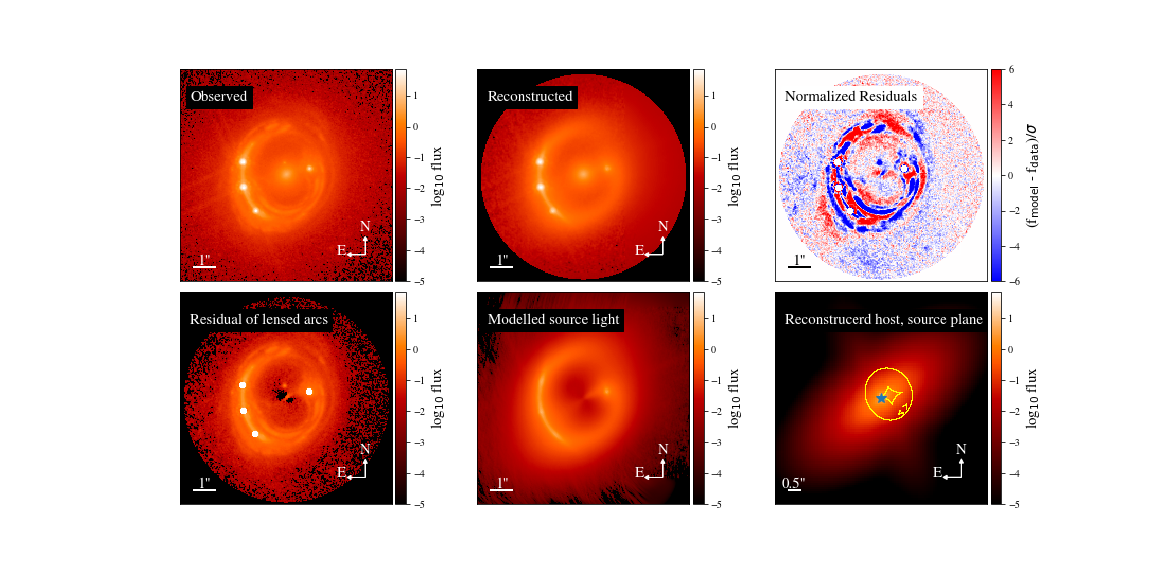
\includegraphics[trim = 40mm 25mm 40mm 25mm, clip, width=0.5\textwidth]{fig/RXJ1131_inference.png}}\\
\subfloat[WFI2033]{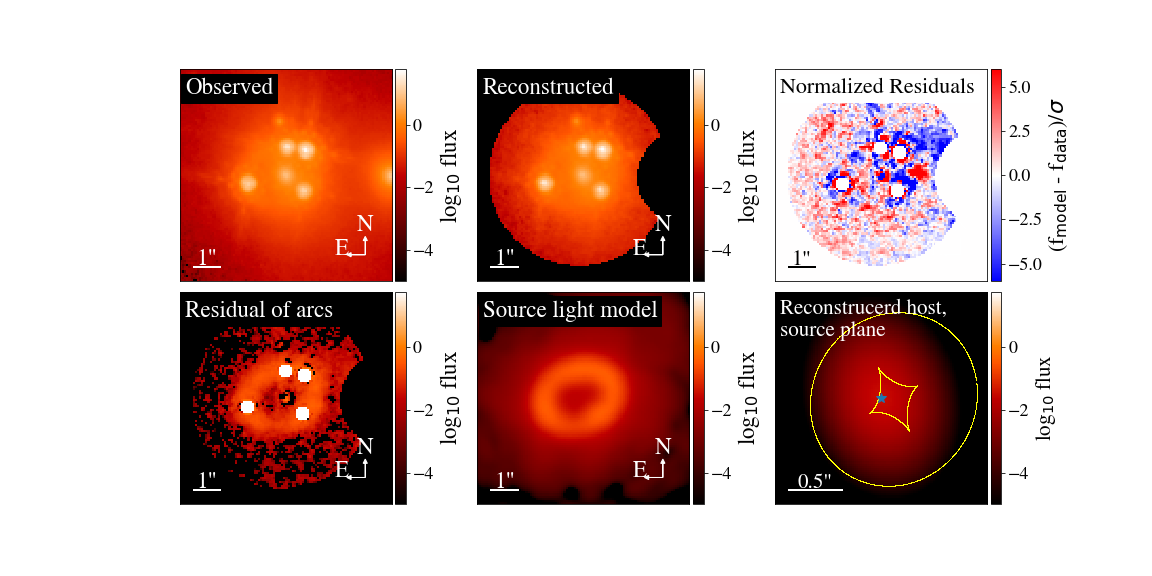
\includegraphics[trim = 40mm 25mm 40mm 25mm, clip, width=0.5\textwidth]{fig/WFI2033_inference.png}}&
\subfloat[SDSS1206]{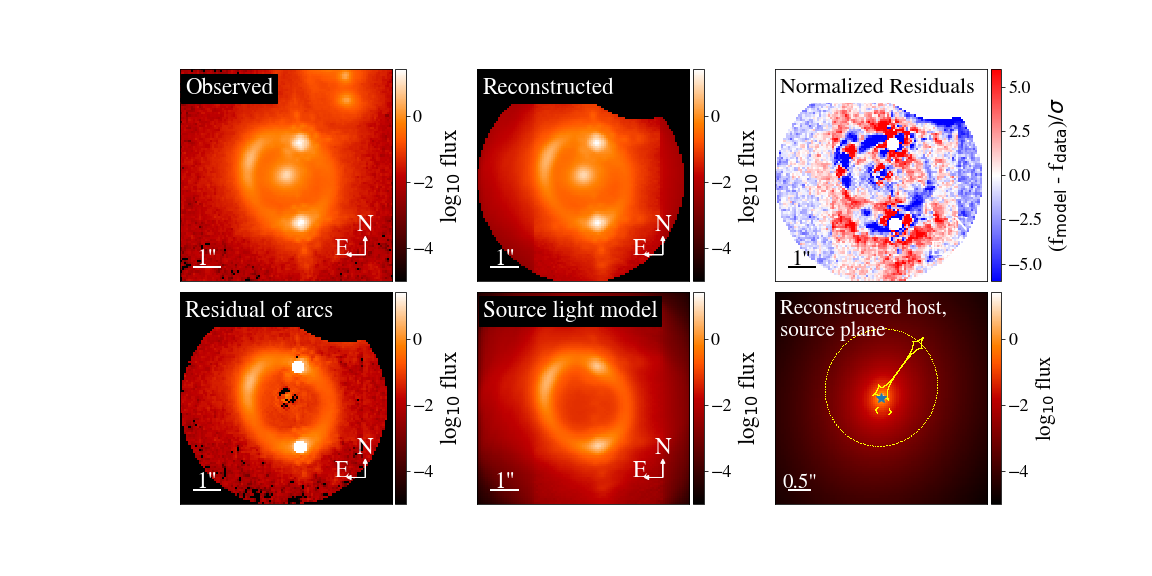
\includegraphics[trim = 40mm 25mm 40mm 25mm, clip, width=0.5\textwidth]{fig/SDSS1206_inference.png}}\\
\subfloat[HE1104]{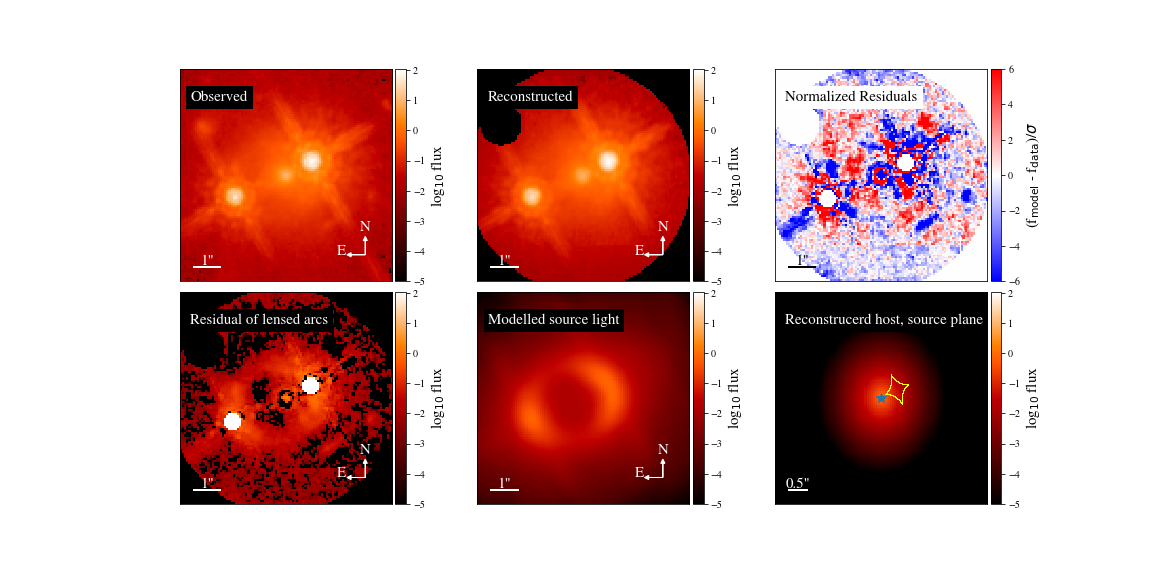
\includegraphics[trim = 40mm 25mm 40mm 25mm, clip, width=0.5\textwidth]{fig/HE1104_inference.png}}&
\subfloat[SDSS0246]{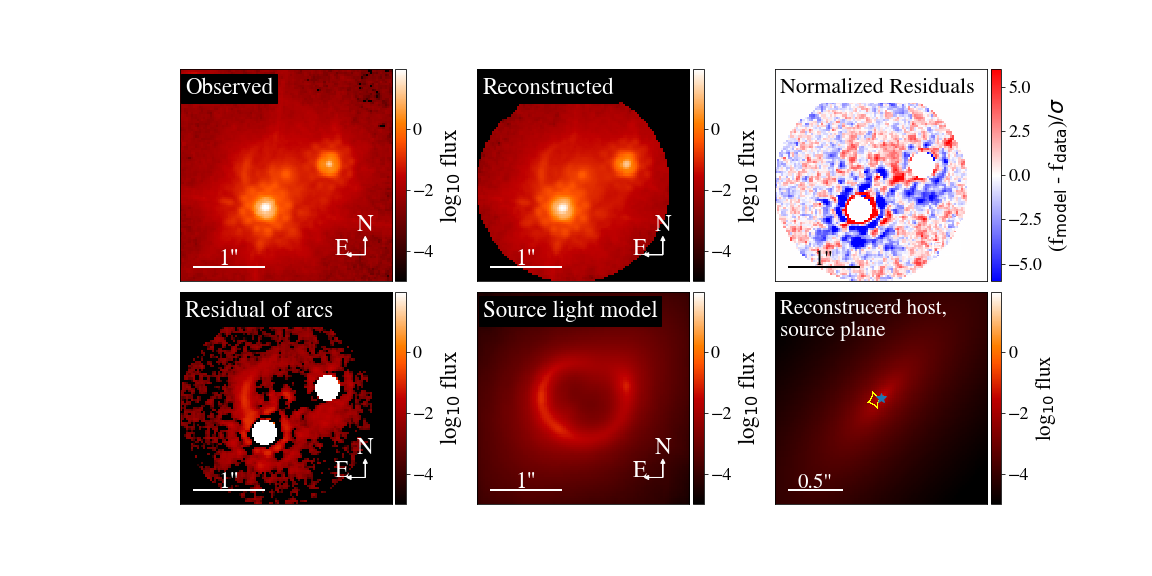
\includegraphics[trim = 40mm 25mm 40mm 25mm, clip, width=0.5\textwidth]{fig/SDSS0246_inference.png}}\\
\subfloat[HS2209]{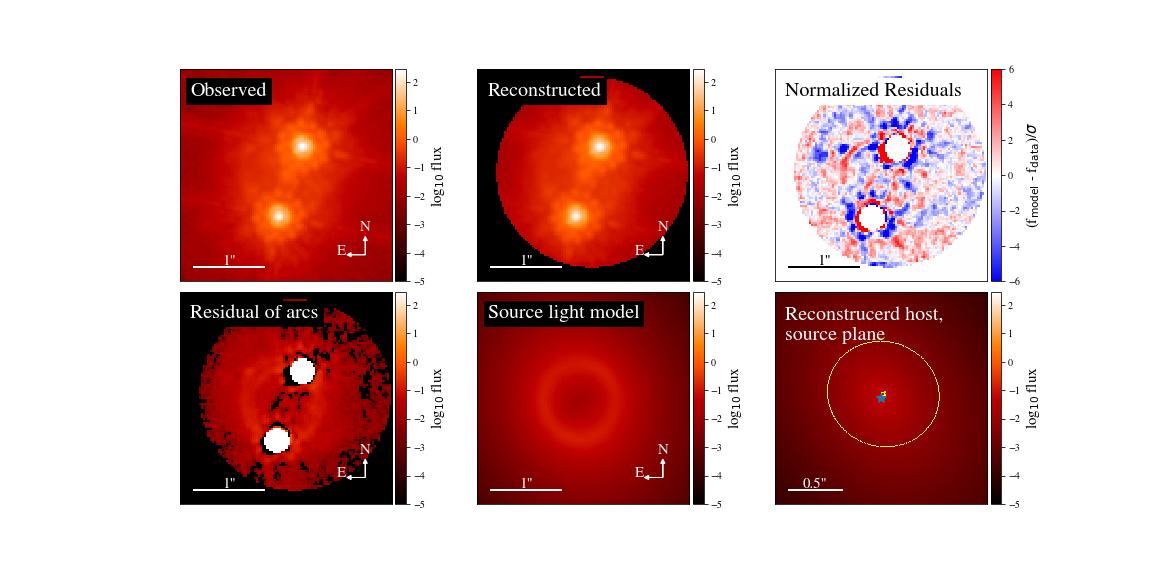
\includegraphics[trim = 40mm 25mm 40mm 25mm, clip, width=0.5\textwidth]{fig/HS2209_inference.png}}&
\subfloat[HE0047]{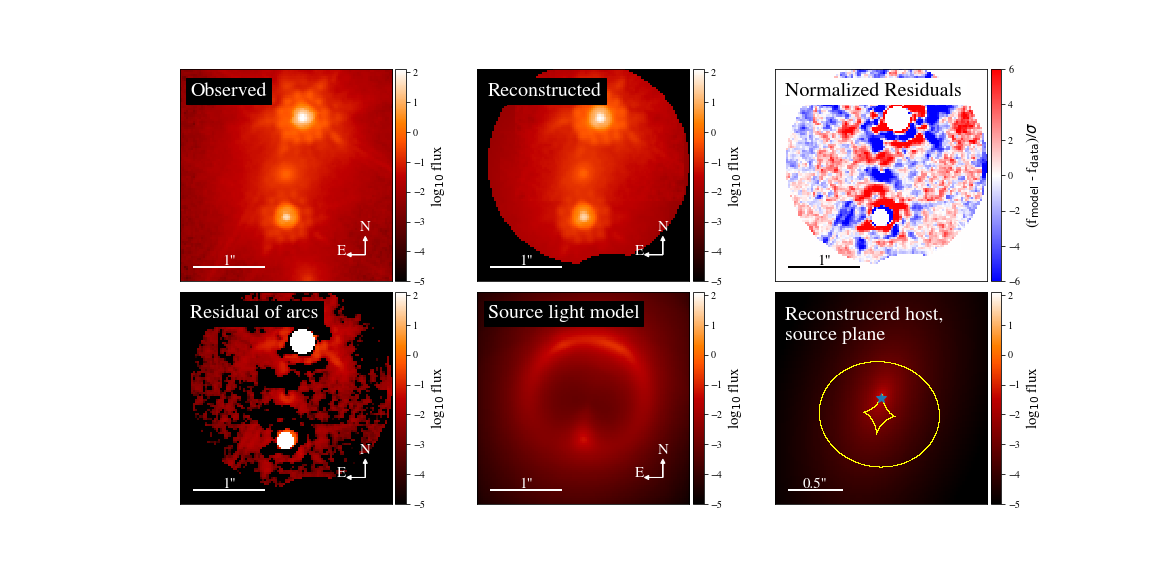
\includegraphics[trim = 40mm 25mm 40mm 25mm, clip, width=0.5\textwidth]{fig/HE0047_inference.png}}\\
\end{tabular}
\caption{\label{fig:image_inference} 
Illustrations of the inference for each system. On the top: (left to right): . On the bottom: (left to right.) }
\end{figure*} 

\subsubsection{RXJ1131}
The image of RXJ1131 observed with ACS/F814W has been well studied in many reference. The host galaxy of this system is lensed to a spacious arc with a boundary line between the dominated area of bulge and disk could be clearly seen. Thus, we set the host galaxy is composed of two \sersic\ with index value $n$ fixed to $1$ and $4$ to mimic the light distribution of the disk and bulge, respectively. Besides, same as suyu[], we consider the perturbations by the small object ($0\farcs{5}$ in the north) and fitting as the SIS and \sersic\ for its mass and light, respectively.

The inference of the RXJ1131 is based on 4 initial PSFs which is summarized in Table~\ref{tab:host_measure}, with the best-fit result drawn in Figure~\ref{fig:image_inference}-(b).

We also compare our measurement to the previous reconstructions in Ding. Based on the reconstructions by Suyu[], the inference of the host magnitude by Ding[] is $mag_{\rm bulge} = 21.81 \pm 0.28$ and $mag_{\rm disk} = 20.07\pm0.06$. Compared to our inference in Table~\ref{tab:host_measure}, the bulge flux is very consistent, however, while our inferred disk is brighter by $\sim 0.5$ mag. \ding{Some discussion of this offset.}

\subsubsection{WFI2033}
WFI2033 is the last quads which has also been carefully studied recently in Ken[]. There is a satellite galaxy in the north. However, as noted by Ken[], it has a much smaller mass than the main deflector, thus we ignore its influence on the magnification but only fit its light using a \sersic\ model. There are in total of 8 PSF stars are selected to modelling this system.

The final inference are presented in Table~\ref{tab:host_measure} and Figure~\ref{fig:image_inference}-(c). We also compare the inference to the reconstructions by Ken. Fitting their reconstruction as a \sersic\ profile, we have inferred that $mag = 21.98 \pm 0.15$ which is also consistent to our inference.

\subsubsection{SDSS1206}
SDSS1206 is a special system -- the AGN is a doubly images while most of the host is falls inside the inner caustic thus being quadruply imaged. We consider the galaxy triplet group at the north-west and use a single SIS model to denote their over all mass perturbations. Moreover, as noted by Simon[], a sub-clump is located in the north which is hardly visible  (i.e., Figure 1 in that paper). We model it as a SIS mass model and circular \sersic\ light model with joint centroids. Though we see the visible residuals in the fitted arcs using a single \sersic\ model, we find a double \sersic\ could help significantly improve the goodness of the fitting. Thus, we adopt the single \sersic\ model in our final inference. 

Due to limit of stars in the filed of view, there are only 2 stars available as initial PSF. To expand the volume of choice options, we also take the stack of the two bright stars as derived by Simon[] as a third initial PSF. Finally, the results are presented in Table~\ref{tab:host_measure} and Figure~\ref{fig:image_inference}-(d).
\todo{Ask Simon for the reconstruction image to compare.}


\subsubsection{HE1104}
As a typical doubly lensed image, the lens model of HE1104 is modelled by us for the first time. We have selected in total of 5 initial PSFs to perform the fitting. The inference of the image is presented in Table~\ref{tab:host_measure} and Figure~\ref{fig:image_inference}-(e).  With the best-fitting model, the lensed arcs could be clearly seen from the bottom-left panel, indicating a strong evidence of the detection of the host.

\subsubsection{SDSS0246}
Imaged with WFC3-UVIS/F814W, the resolution of the data is much higher. However, the arc is much fainter compare to the IR band and the available pixels that could be used to fitting the arc is quite limited. With in total 3 initial PSF selected, the host is successfully reconstructed as shown in Figure~\ref{fig:image_inference}-(f) with inference list in Table~\ref{tab:host_measure}. A template of 0.625 Gyr stellar population would be adopt.

\subsubsection{HS2209}
HS2209 imaging data have two visits. We modelled both two visited drizzling data.
The inference of this system is summarized in Figure~\ref{fig:image_inference}-(g). \ding{The host magnitude might be overestimated. The QSO is over bright with a positive background light. Xuheng is Re-fitting this image.}

\subsubsection{HE0047}
HE0047 is the most challenging system in our sample. The results, based on three PSFs, are summarized in Figure~\ref{fig:image_inference}-(f) and Table~\ref{tab:host_measure}. From the subtracted-everything-except-arc image, the lensed host is only half-seen among the large residuals. Thus, the inference of the HE0047 should be taken with larger scatters, or as upper limit.

\begin{table*}
\renewcommand{\arraystretch}{1.25}
%\setlength{\tabcolsep}{20pt}
\centering
  \begin{threeparttable}
\caption{Summary of lensed AGN inference.}\label{tab:host_measure}    
%\resizebox{12cm}{!}{
     \begin{tabular}{cccccccc}
\hline     
(1) & (2) & (3) & (4) & (5) & (6) & (7) & (8) \\    
Object ID & intrinsic Magnitude & Magnitude & Flux Ratio (to Total) & \reff\ & \sersic\ $n$ & adopted AGE & $\log (M_{*}$)  \\
 & (source plane) & (image plane) & ($\%$) & (arcsec) & & (Gyr) & (M$_{\odot}$) \\ \hline
HE0435 & $21.49\substack{+0.40\\-0.29}$ & $18.58\substack{+0.30\\-0.23}$ & $36.0\pm11.1$ & $0.28\pm0.02$ & $2.71\pm0.20$ & $1.50$ & $10.91\substack{+0.12\\-0.16}$ \\
RXJ1131$_{\rm bulge}$ & $21.80\substack{+0.23\\-0.19}$ & $18.70\substack{+0.07\\-0.06}$ & $7.1\pm1.4$ & $0.13\pm0.02$ & fix to 4 & $3.00$ & $10.39\substack{+0.08\\-0.09}$ \\
RXJ1131$_{\rm disk}$ & $19.33\substack{+0.17\\-0.15}$ & $17.14\substack{+0.08\\-0.07}$ & $69.2\pm10.1$ & $0.90\pm0.06$ & fix to 1 & $1.50$ & $11.08\substack{+0.06\\-0.07}$ \\
WFI2033 & $21.78\substack{+0.28\\-0.23}$ & $19.07\substack{+0.35\\-0.26}$ & $19.6\pm4.5$ & $0.28\pm0.02$ & $0.52\pm0.01$ & $0.62$ & $10.51\substack{+0.09\\-0.11}$ \\
SDSS1206 & $21.31\substack{+0.23\\-0.19}$ & $18.30\substack{+0.05\\-0.05}$ & $33.3\pm6.4$ & $0.11\pm0.02$ & $4.57\pm0.53$ & $0.62$ & $10.77\substack{+0.08\\-0.09}$ \\
HE1104 & $21.25\substack{+0.16\\-0.14}$ & $19.16\substack{+0.02\\-0.02}$ & $14.0\pm2.0$ & $0.27\pm0.02$ & $1.05\pm0.04$ & $0.63$ & $11.05\substack{+0.06\\-0.07}$ \\
SDSS0246 & $23.44\substack{+0.28\\-0.22}$ & $20.85\substack{+0.08\\-0.07}$ & $4.0\pm0.9$ & $0.44\pm0.08$ & $4.96\pm0.08$ & $0.63$ & $10.75\substack{+0.09\\-0.11}$ \\
HS2209 & $20.72\substack{+0.26\\-0.21}$ & $19.20\substack{+0.04\\-0.04}$ & $12.5\pm2.7$ & $1.96\pm1.28$ & $3.15\pm1.40$ & $1.00$ & $11.04\substack{+0.08\\-0.10}$ \\
HE0047 & $22.92\substack{+0.48\\-0.33}$ & $20.37\substack{+0.20\\-0.17}$ & $2.3\pm0.8$ & $0.32\pm0.15$ & $4.18\pm0.75$ & $0.62$ & $10.91\substack{+0.13\\-0.19}$ \\
\hline
\end{tabular}
%}
\begin{tablenotes}
      \small
      \item Note: $-$ If any
\end{tablenotes}    
\end{threeparttable}
\end{table*}


\section{Results}\label{sec:result}
In this section, we describe the approaches and assumptions to adopt the stellar population to our sample. We then derive their stellar mass of our sample and study the  the scaling relation by connecting them to their \mbh. We compare our measurements by our sample to the ones in the literature to study their evolution.

\subsection{Stellar population and mass}\label{sec:mstar}
%[] Color inference for the first three cases to decide their stellar template. 
Besides the band we imaging data at the given band we studied in last section, some of the systems also have other band observations by the \hst, which provides the color information of the host galaxy. Given that the other band data has less exposure time with lower single to noise level, we highlight that we only study the color to find a decent stellar template. Then, it would be adopted to the host photometry obtained in last section to infer the final stellar mass.

{\bf HE0435} ~ Besides the imaging data by F160W, this system has also been observed by the \hst\ through F814W and F555W band. We adopted the same approach to modelling the data separately at these two band. % The inferred host magnitudes are xxx and xxx, respectively.
Considering that the lensed host in the image plane is majorly inferred by the subtraction of the AGNs and deflectors light, which it is less dependent on the lens model. We expect it can be obtained with more accuracy. Thus, we infer the color based on the magnitude of the lensed arcs in the image plane. We use {\sc Gsf} code to fit the magnitude of the lensed host and find a 1.5 Gyr stellar template with solar metallicity could well match this color. More details of the information could be found in the Appendix~\ref{app:HE0435}.

{\bf RXJ1131} ~ For this system, the lensed arc is very extended in the image plane which is resolved to the AGNs, one could directly perform the SED fitting of the arc in the image plane. Combining the \hst\ imaging data through three filter F814W and F555W and F160W, we inference the color and we adopt the stellar templates 3 Gyr and 1.5 Gyr with solar metallicity stellar to its bulge and disk, respectively (see Appendix~\ref{app:RXJ1131} for the inference).

{\bf WFI2033} ~ Besides the F160W filter, four other filters including F125W, F140W, F555W, F814W are also available in the \hst\ archive, which has been employed to obtain the color of the host galaxy. We perform the lens model inference for all the filter and infer the host color through five band in the image plane. We find a stellar template with 0.625 Gyr could well match their color (Appendix~\ref{app:WFI2033}).

{\bf HE1104 and the other systems} ~ The imaging data of HE1104 has been observed through F555W and F814W band. However, given limited exposure time, the signal of the lensed arcs is too faint to be detected at this two bands. Due to this limitation, we couldn't infer the color of the host for HE1104. For this case, the other systems, we adopt the criteria by Ding2020[] to assign their stellar population, i.e., the 1 Gyr and 0.625 Gyr stellar population would be adopted for systems as $z<1.44$ and $z>1.44$, respectively.

A summary of the adopted stellar populations is given in Table~\ref{tab:host_measure}, column~(7). Applying these templates to the filter magnitudes obtained in last section, we obtain the stellar mass of our system. Considering that we have obtained very consistent host photometry for the HE0435, RXJ1131 and WFI2033 to previous results using the independent approach, the fidelity of the inferred magnitude are considered to be high. The uncertainty of the \mstar\ estimation are considered as the typical level $0.2$~dex. Same as the comparison, we expect that the uncertainty of the \mbh\ would dominate the error budget in the overall scaling relation obtained in next section.

\subsection{The \mbh-\mstar\ relation}\label{sec:relation}
Having obtained the \mstar\ of each individual system, we combine them with their \mbh\ to reveal the scaling relations. We expect to compare our high redshift lensed sample to the comparison sample as introduced in Section~\ref{sec:sample_select}. We plot the entire measurement together with and present in Figures~\ref{fig:scaling_relation}-(a). Following~\citet{Ding2020}, we fit the \mbh-\mstar\ data with a linear relation as:
\begin{eqnarray}
\label{eq:MMlocal}
\log \big( \frac{\mathcal M_{\rm BH}}{10^{7}M_{\odot}})= \alpha + \beta \log(\frac{M_*}{10^{10}M_{\odot}}).
\end {eqnarray}
We find that our lensed systems appeared to have a slimier offset to the local relations which is consistent to the 32 QSOs by~\citet{Ding2020} at similar redshift range.

To this evolution trend based on the sample redshift, we parameterize the evolution term as the linear relation by:
\begin{eqnarray}
\label{eq:offset}
\Delta \log \mathcal M_{\rm BH}= \gamma \log (1 + z),
\end{eqnarray} 
from which we recover the offset plot, i.e., Figure~8, in~\citet{Ding2020}. We then add the measurements by our lensed systems and show in Figure~\ref{fig:scaling_relation}-(b). We find that the evolution of the offset our sample are well matched to the evolution trend as discovered by the previous inference. Given that we only obtain the measurements from eight lens systems, it is insufficient to fit the offset value quantitively. Nevertheless, the obvious consistency between the sample confirm the fidelity of our measurement and verify previous offset conclusions by~\citet{Ding2020}.

\begin{figure*}
\centering
\begin{tabular}{c c}
{\includegraphics[height=0.5\textwidth]{fig/MBH-Mstar.pdf}}&
{\includegraphics[height=0.5\textwidth]{fig/MBH-Mstar_vz.pdf}}\\
\end{tabular}
\caption{\label{fig:scaling_relation} 
\todo{This Figures are still ugly so far, which need to be updated.}}
\end{figure*} 

\section{Discussion and Conclusion}
[] This work confirm the bright future of lensing.

Finally, we did not consider the selection effect. Besides the mass function, the selection function of the lensed AGNs is also non-trivial. We note that these effects will have to be modelled in the future if the lensed sample is used to infer the evolution. 

Look at the future? JWST and TDCOSMO will extend the sample size.


\section*{Acknowledgements}

The Acknowledgements section is not numbered. Here you can thank helpful
colleagues, acknowledge funding agencies, telescopes and facilities used etc.
Try to keep it short.

%%%%%%%%%%%%%%%%%%%%%%%%%%%%%%%%%%%%%%%%%%%%%%%%%%

%%%%%%%%%%%%%%%%%%%% REFERENCES %%%%%%%%%%%%%%%%%%

% The best way to enter references is to use BibTeX:

\bibliographystyle{mnras}
\bibliography{reference} % if your bibtex file is called example.bib


% Alternatively you could enter them by hand, like this:
% This method is tedious and prone to error if you have lots of references
%\begin{thebibliography}{99}
%\bibitem[\protect\citeauthoryear{Author}{2012}]{Author2012}
%Author A.~N., 2013, Journal of Improbable Astronomy, 1, 1
%\bibitem[\protect\citeauthoryear{Others}{2013}]{Others2013}
%Others S., 2012, Journal of Interesting Stuff, 17, 198
%\end{thebibliography}

%%%%%%%%%%%%%%%%%%%%%%%%%%%%%%%%%%%%%%%%%%%%%%%%%%

%%%%%%%%%%%%%%%%% APPENDICES %%%%%%%%%%%%%%%%%%%%%

\appendix

\section{Color inference of the host}
We describe the details of the stellar population inference in this section. The template would be then adopted to the photometry by Section~\ref{sec:photometry} to infer the stellar mass.
\subsection{HE0435}\label{app:HE0435}
The HE0435 system are also modelled through ACS/F814W and ACS/F555W (GO-9744; PI: C. S. Kochanek). We derive the magnitude of the lensed galaxy and infer the color of the host in the image plane. We illustrate the lens model for the other two band in Figure~\ref{fig:app_HE0435}. The inferred magnitude of the host galaxy in the image plane is quite robust. Having obtained the magnitude of the lensed host at three band, we use {\sc gsf} package to select the best stellar population from a range of [0.625, 0.8, 1.0, 1.5, 2.0, 3.0] Gyr with solar metallicity. Finally, a template with ago of 1.5 Gyr is selected.


\begin{figure*}
\centering
\subfloat[HE0435 F555W]{\includegraphics[ width=0.8\textwidth]{fig/HE0435_f555w_inference.pdf}}\\
\subfloat[HE0435 F814W]{\includegraphics[ width=0.8\textwidth]{fig/HE0435_f814w_inference.pdf}}
\caption{\label{fig:app_HE0435} 
Illustrations of the inference of HE0435 at the other two band. }
\end{figure*} 


\subsection{RXJ1131}\label{app:RXJ1131}
Using the three band data including  ACS/F814W and ACS/F555W and NIC2/F160W (GO-9744; PI: C. S. Kochanek), we preform the SED fitting in the imaging plane directly pixel by pixel in Figure~\ref{fig:app_RXJ1131}. \ding{This part is actually done by Takahiro in~\citep{Ding2017b}. The image of the fitted age looks noisy, but it is in the range of the [9.25 - 9.50] (logAge), i.e. [1.5, 3.0] (Gyr). We can remove this A2 but only mention the fitting is done 2017 in that paper.}
\begin{figure}
\centering
{\includegraphics[width=0.25\textwidth]{fig/map_age_zRXJ_1131.pdf}}\\
\caption{\label{fig:app_RXJ1131} 
Illustrations of the SED fitting of the galaxy age pixel by pixel.  }
\end{figure} 

\subsection{WFI2033}\label{app:WFI2033}
WFI2033 is also observed by other four band data including WFC3/F125W (GO-12874; PI: D. Floyd), WFC3/F140W (GO-13732; PI: A. Nierenberg), ACS/F555W+F814W  (GO-9744; PI: C. S. Kochanek). The data quality by F125W is limited by its exposure time; and the host information is not well extracted. We does not take it into account in the color inference. 
Similar to Section~\ref{app:HE0435}, the lensed color of WFI2033 has been modelled through five band. The lensed models are presented in the~Figure~\ref{fig:app_WFI2033}.

\begin{figure*}
\centering
\subfloat[WFI2033 F125W \todo{remove arrows}]{\includegraphics[ width=0.8\textwidth]{fig/WFI2033_f125w_inference.pdf}}\\
\subfloat[WFI2033 F140W \todo{remove arrows}]{\includegraphics[ width=0.8\textwidth]{fig/WFI2033_f140w_inference.pdf}}\\
\subfloat[WFI2033 F555W]{\includegraphics[ width=0.8\textwidth]{fig/WFI2033_f555w_inference.pdf}}\\
\subfloat[WFI2033 F814W]{\includegraphics[ width=0.8\textwidth]{fig/WFI2033_f814w_inference.pdf}}
\caption{\label{fig:app_WFI2033} 
Illustrations of the inference of WFI2033 at the other two band.  }
\end{figure*} 
%%%%%%%%%%%%%%%%%%%%%%%%%%%%%%%%%%%%%%%%%%%%%%%%%%


% Don't change these lines
\bsp	% typesetting comment
\label{lastpage}
\end{document}

% End of mnras_template.tex